%!TEX root = report.tex
\exercise{Filtering}
\setcounter{subsection}{0}
\subsection{Gaussian lowpass filter}
We have implemented the Gaussian lowpass filter according to Eq. 4.8-7 in the function \texttt{IPgaussian} in the following function:
\matlabexternal{IPgaussian.m}
By default this function acts as the Gaussian lowpass filter, but if the flag \texttt{lowpass} is set to false, it will act as a Gaussian highpass filter. By setting the values of \texttt{P} and \texttt{Q} the size of the output image can be modified according the user's wishes.
\subsection{IPftfilter}
We have written a function \texttt{IPftfilter} that performs filtering in the frequency domain. The code that does this is the following code:
\matlabexternal{IPftfilter.m}
This function when called with just the image and the cutoff frequency $d_0$ the function will return a lowpass Gaussian filtered image with the size of the original image. It transforms the image to the frequency domain and subsequently does a point-wise multiplication with the Gaussian filter. After transforming it back to the spatial domain, the filtered image is obtained.
\subsection{Lowpass characters}
We have loaded the image \texttt{characters.tif} using the function \texttt{readDoubleImage} and called it with the cutoff frequencies 5, 20, 30, 50 and 100. We believe with these values the images in Fig. 4.48 in the book are best approximated. The resulting images are in figure~\ref{fig:lowChars}.
\begin{figure}[ht]
 \centering
 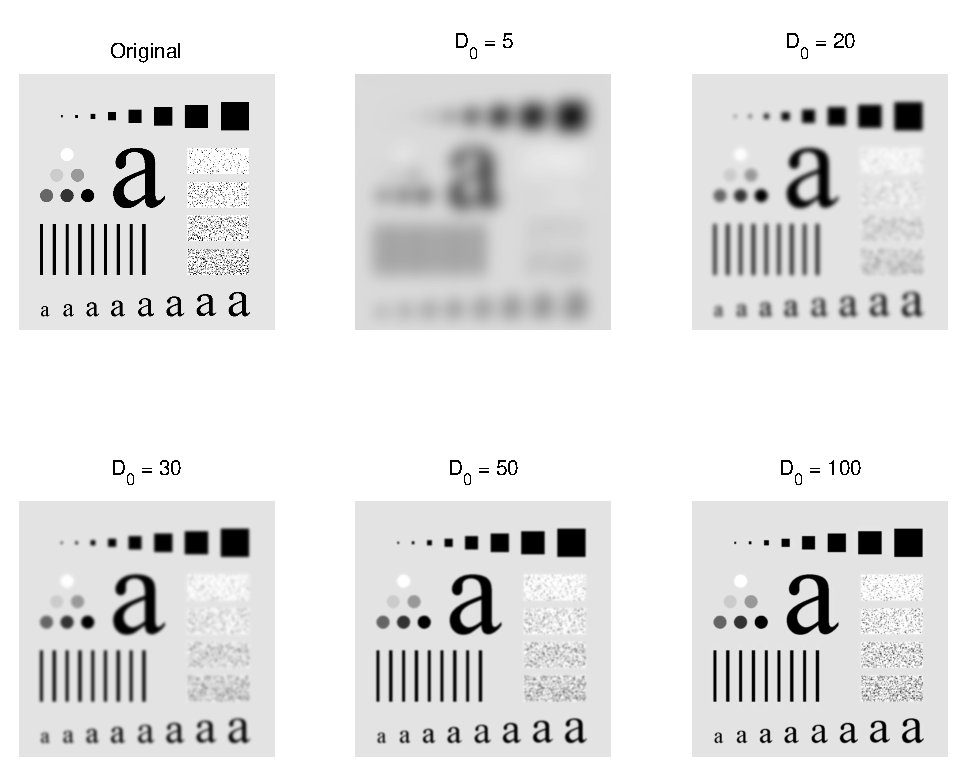
\includegraphics{characters_low_pass.eps}
 \caption{Testing the highboost filter for several options of $k$. The image with $k = 4.5$, bottom-right, is the closest to image 3.40(e) in the book.}
 \label{fig:lowChars}
\end{figure}
\subsection{Gaussian highpass filter}
We also have implemented the Gaussian highpass filter. This turns out to be the complement of the Gaussian lowpass filter and therefore we have implemented that function as such in the function \texttt{IPgaussian}. This makes sense because instead of passing low frequencies you want high frequencies and therefore low frequencies must be eliminated. The highpass filter can be used by calling \texttt{IPgaussian} and setting the flag \verb lowpass  to false.
\subsection{Highpass characters}
The same image is loaded here as in exercise 3c, but instead a highpass filter is applied to approximate image 4.56 in the book. To approximate these images we have used the cutoff frequencies 30, 60 and 100. We have chosen these cutoff frequencies as they are mentioned in the caption of image 4.56 and, as figure~\ref{fig:highChars} illustrate, they are duplicates of the image in the book.  
\begin{figure}[ht]
 \centering
 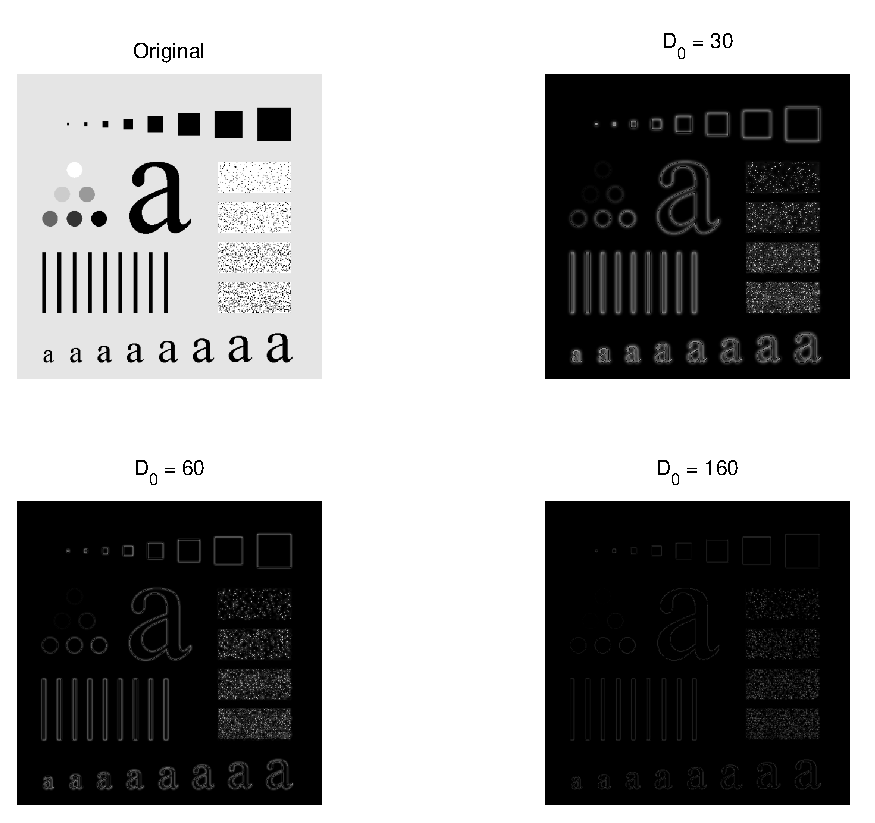
\includegraphics{characters_high_pass.eps}
 \caption{Testing the highboost filter for several options of $k$. The image with $k = 4.5$, bottom-right, is the closest to image 3.40(e) in the book.}
 \label{fig:highChars}
\end{figure}
\clearpage